\chapter{Análisis de Resultados}
\section{Resultados}

Se ha logrado mediante la implementación de un sistema de inversor de voltaje alcanzar voltajes de hasta 2 KV a una potencia de 40w, voltaje controlado digitalmente por un computador. Se ha desarrollado un código en root CERN para encontrar el voltaje RMS de nuestro voltaje de salida. Nuestras mediciones realizadas arrojaron las siguientes distribuciones para diferentes voltajes sin carga alguna. \\

\begin{figure}[H]
\centering
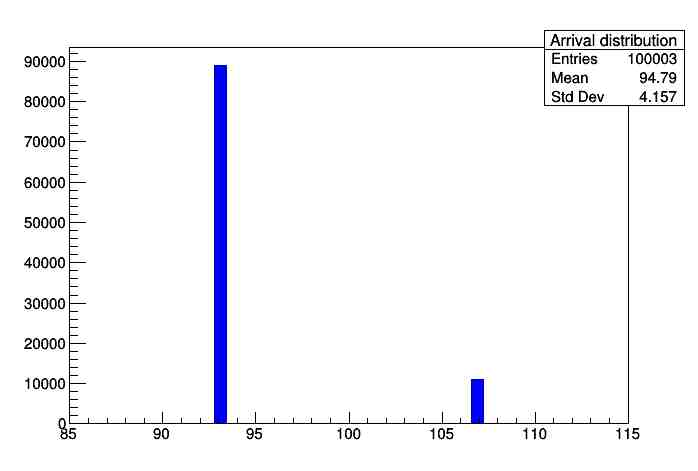
\includegraphics[width=12cm]{Capitulo4/93v.jpg}
\caption{Salida alto voltaje sin carga a 93V.}
\end{figure}

\begin{figure}[H]
\centering
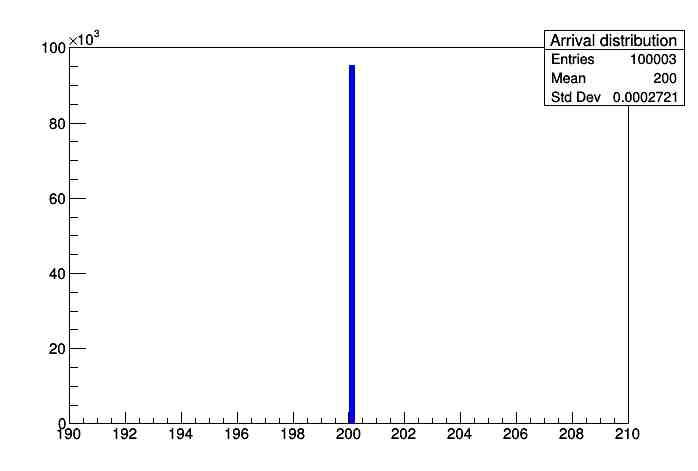
\includegraphics[width=12cm]{Capitulo4/200v.jpg}
\caption{Salida alto voltaje sin carga a 200V.}
\end{figure}

\begin{figure}[H]
\centering
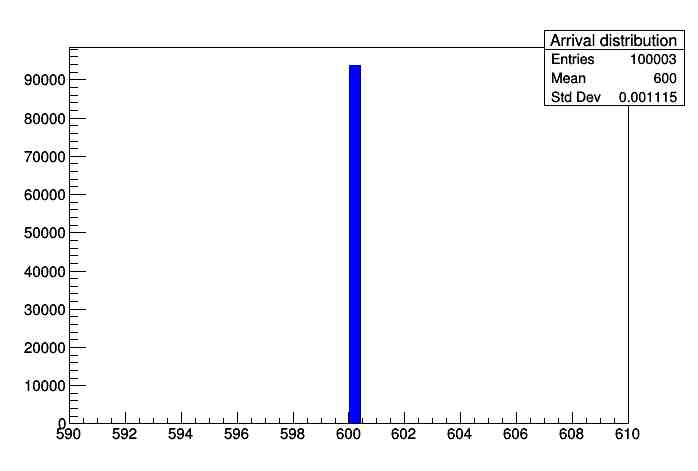
\includegraphics[width=12cm]{Capitulo4/600v.jpg}
\caption{Salida alto voltaje sin carga a 600V.}
\end{figure}

\begin{figure}[H]
\centering
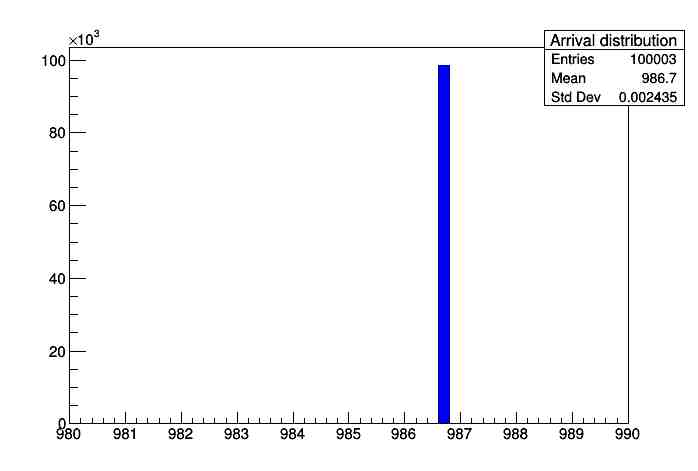
\includegraphics[width=12cm]{Capitulo4/986v.jpg}
\caption{Salida alto voltaje sin carga a 986V.}
\end{figure}
\newpage

Como observamos se ha obtenido voltajes sin perturbaciones y con relativo bajo rizo asociado a él. Se realizaron diez mil mediciones por cada distribución y a partir de ella podemos observar un voltaje RMS de 4.15V a 93V, 0.00027V para 200V, 0.0011V para 600V y 0.0024V para 986V respectivamente. \\

Utilizando la ecuación 2.6 podemos calcular el rizo asociado a la señal. Se observa en la tabla los siguientes resultados de nuestras mediciones con sus variables correspondientes. 

\begin{table}[H]
\begin{tabular}{@{}llll@{}}
\toprule
Voltaje   & Frecuencia & Dutty & Riso \\ \midrule
93  & o.o        & 0.0   &  0.0\\
200 & 0.0        & 0.0   &   0.0\\
600 & 0.0        & 0.0   &   0.0\\
986 & 0.0        & 0.0   &   0.0\\ \bottomrule
\end{tabular}
\end{table}


Los resultados indican que se ha desarrollado una fuente con requerimientos suficientes para trabajos de laboratorio. 